% ============================================
% VCP：面向小样本目标检测的单阶段余弦分类器与原型学习
% 中文翻译稿
% ============================================

\documentclass[conference]{IEEEtran}
\IEEEoverridecommandlockouts

\usepackage{cite}
\usepackage{amsmath,amssymb,amsfonts}
\usepackage{graphicx}
\usepackage{booktabs}
\usepackage{multirow}
\usepackage{hyperref}
\usepackage{stfloats}
\usepackage{textcomp}
\usepackage{xeCJK}
\setCJKmainfont{SimSun}

\begin{document}

\title{VCP：面向小样本目标检测的单阶段余弦分类器与原型学习}

\author{\IEEEauthorblockN{费祥\textsuperscript{1}}
\IEEEauthorblockA{\textit{曲阜师范大学 工学院} \\
山东 日照 \\
Fly39@qfnu.edu.cn}
\and
\IEEEauthorblockN{李梦茹\textsuperscript{2}}
\IEEEauthorblockA{\textit{曲阜师范大学 工学院} \\
山东 日照 \\
13864085521@qfnu.edu.cn}
\and
\IEEEauthorblockN{黄晋铭\textsuperscript{3*}}
\IEEEauthorblockA{\textit{曲阜师范大学 工学院} \\
山东 日照 \\
huangjm@qfnu.edu.cn}
\and
\IEEEauthorblockN{刘建波\textsuperscript{4}}
\IEEEauthorblockA{\textit{歌尔股份有限公司 技术部} \\
山东 潍坊 \\
2374622833@qq.com}
\and
\IEEEauthorblockN{张晓夫\textsuperscript{5}}
\IEEEauthorblockA{\textit{山东自由光学科技有限公司 技术部} \\
山东 潍坊 \\
fly39@icloud.com}
\and
\IEEEauthorblockN{徐小皎\textsuperscript{6}}
\IEEEauthorblockA{\textit{山东慧米智能科技有限公司 技术部} \\
山东 日照 \\
17604705924@163.com}
\thanks{本文受山东省重点研发计划（2025TSGCXTHG031）和国家重点研发计划（2021YFE0193900）资助。通讯作者：黄晋铭（huangjm@qfnu.edu.cn）。}
}

\maketitle

\begin{abstract}
小样本目标检测（FSOD）目前主要基于 Faster R-CNN 等两阶段架构，而工业部署中广泛使用的 YOLO 系列单阶段检测器缺乏系统性的小样本研究。本文提出 VCP（Visual-Cosine-Prototype），将 YOLO11s 与余弦分类器及原型学习相结合，在 TFA 协议下构建单阶段 FSOD 框架。在 PASCAL VOC 数据集上，VCP 在 10-shot 设定下以仅 9.5M 参数量（约为竞争方法的 1/6）取得 72.2\% 的 mAP50（三划分均值）；然而在 MS COCO 上，同一方法不如标准微调。通过对 24 组实验进行系统的精确率--召回率分解，我们发现余弦分类器表现为一种\textit{召回增强器}，持续将预测推向高召回、低精确率的方向。我们提出 P-R Tradeoff 假说：净收益取决于基线召回空间与数据集特定的 P-R 权衡比的乘积，解释了 VOC 与 COCO 上的效果反转。我们还探索了 Florence-2 语义描述作为轻量级辅助先验（+0.5 pp，零 VLM 推理开销）。VCP 运行速度达 54.4 FPS，比两阶段 FSOD 方法快 4--5 倍。
\end{abstract}

\begin{IEEEkeywords}
小样本目标检测，单阶段检测器，余弦分类器，原型学习，召回增强器
\end{IEEEkeywords}

\section{引言}

小样本目标检测（FSOD）旨在仅凭每个类别极少标注样本检测新类别。FSCE~\cite{sun2021fsce} 和 DeFRCN~\cite{qiao2021defrcn} 等方法推动了 FSOD 基准的提升，但一个显著共性依然存在：几乎所有现有 FSOD 方法都建立在两阶段 Faster R-CNN~\cite{ren2015faster} 之上，其区域提议网络（RPN）提供了内建的前景过滤机制，有效控制了数据稀缺条件下的假阳性。然而在工业部署中，YOLO 家族~\cite{terven2023yolo,jocher2023ultralytics} 因其高实时效率而占据主导地位。这造成了"已发表方法无法部署，已部署系统缺乏研究基础"的脱节。据我们所知，尚无先前工作在标准 TFA 协议下系统研究现代 YOLO 检测器（v8+）的 FSOD 表现。

单阶段 FSOD 的核心挑战在于缺少 RPN 过滤：密集预测范式生成大量低质量候选框，使分类器面临极端的正负样本不平衡。余弦分类器~\cite{wang2020tfa} 通过特征和权重的归一化缓解过拟合，而 Florence-2~\cite{xiao2024florence2} 通过详细的图像描述提供细粒度语义理解。然而，将余弦分类与单阶段 YOLO 检测器结合并系统分析其行为模式，仍是未探索的领域。

我们提出 VCP，将 YOLO11s 的线性分类头替换为由支持集视觉原型初始化的余弦分类器（Proto 模式），并进一步融合 Florence-2 语义描述作为辅助先验（Fused 模式）。在 VOC 上，VCP 以 9.5M 参数量在 10-shot（三划分均值）下取得 72.2\% mAP50，与 60M 参数量的 SOTA 方法具有竞争力；Split 1 达到 74.7\%，超越所有现有两阶段方法。

令人惊讶的是，同一方法在 COCO 上的表现不如标准微调。通过对 24 组实验进行系统 P-R 分解，我们发现余弦分类器作为一种\textbf{召回增强器}，始终以牺牲精确率为代价换取召回率的提升。我们提出\textbf{P-R Tradeoff 假说}来解释这种跨数据集的反转现象。本文贡献如下：(1) 首次在 TFA FSOD 协议下系统探索单阶段 YOLO 检测器；(2) 发现余弦分类器的召回增强器特性并提出 P-R Tradeoff 假说；(3) 具有零推理开销的 VLM 语义原型融合；(4) 提出逐类温度缩放作为轻量级机制，部分抵消召回增强器的精确率损失。

\section{相关工作}

FSOD 已从早期的元学习方法~\cite{huang2025prototype,gao2025decoupling} 过渡到 TFA~\cite{wang2020tfa} 建立的微调范式。FSCE~\cite{sun2021fsce}、DeFRCN~\cite{qiao2021defrcn} 和 KD-DeFRCN~\cite{pei2022kddefrcn} 分别改进了候选框编码、梯度解耦和知识蒸馏。多尺度数据增强~\cite{vu2025multiperspective}、基于检索的域适应~\cite{li2025domainrag} 和边缘优化~\cite{li2021cme} 进一步推动了该领域的发展。这些方法均共享 Faster R-CNN 骨干网络，利用其 RPN 进行候选框质量控制。

单阶段 FSOD 的探索仍极为有限。Meta-YOLO 在 YOLOv2 上采用元学习但依赖高方差划分协议；近期单阶段设计~\cite{chen2025generalized} 在 TFA 协议下探索了对比特征学习。尚无先前工作在 TFA 协议下研究现代 YOLO 检测器（v8+）。我们的语义分支并非作为架构创新提出，而是一种策略选择：小样本视觉原型固有噪声，而详细的 VLM 描述作为互补语义先验来稳定分类器初始化——同时具备关键的零推理开销优势。

CLIP~\cite{radford2021clip} 和 Florence-2~\cite{xiao2024florence2} 等视觉语言模型使得语义原型构建成为可能，而 OWL-ViT~\cite{minderer2022owlvit}、GLIP~\cite{li2022glip} 和 Grounding DINO~\cite{liu2023groundingdino} 推动了开放词汇检测的发展。如何在 FSOD 严格的数据约束（每类 1--10 样本）下有效利用 VLM 原型而不引入过多语义噪声，仍是有待探索的问题。

\section{方法}

\subsection{框架与原型}

VCP 基于 YOLO11s 构建，将其标准线性分类头替换为余弦相似度分类器（图~\ref{fig:framework}）。对于候选框特征 $f\in\mathbb{R}^d$，类别 $c$ 的分类得分为 $s_c=\cos(f,p_c)/\tau$，其中 $p_c$ 为类别 $c$ 的原型，$\tau$ 为可学习温度参数。L2 归一化（$\|f\|=\|p_c\|=1$）确保分类仅依赖于 $f$ 与 $p_c$ 之间的方向对齐，从而缓解有限监督下的过拟合。

\begin{figure*}[t]
\centering
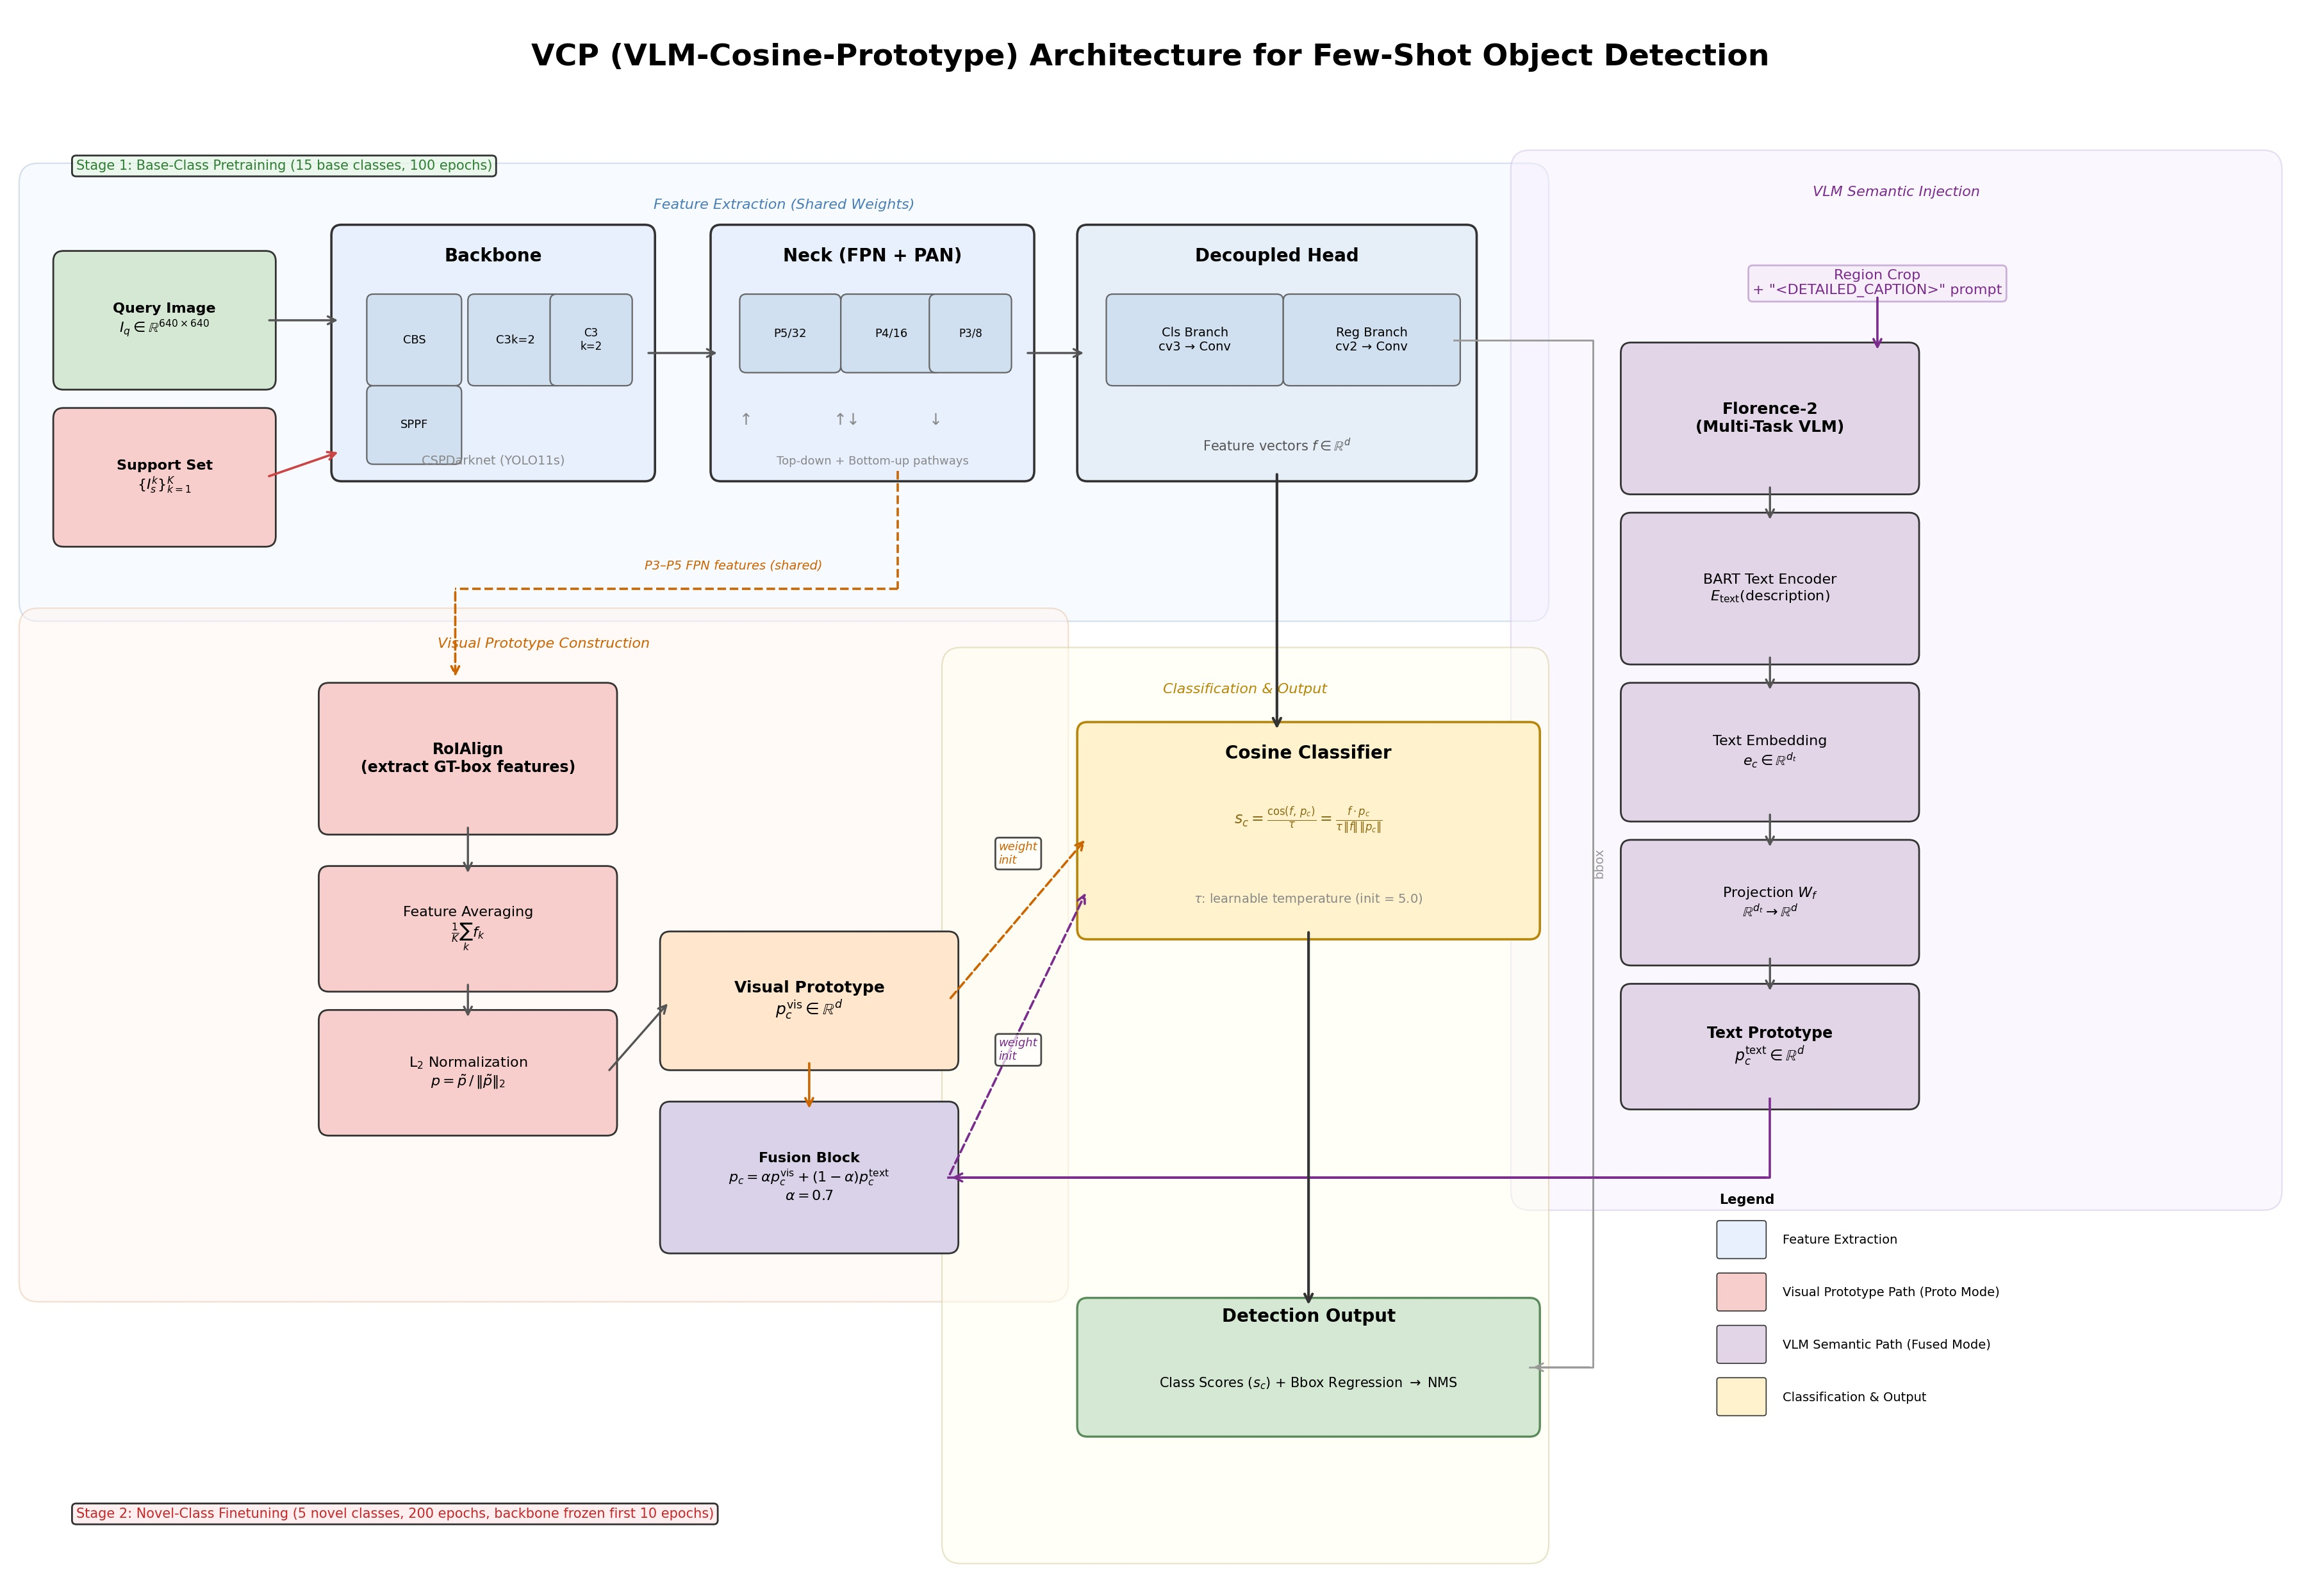
\includegraphics[width=0.88\textwidth]{fig1_framework.jpg}
\caption{VCP 框架：YOLO11s 骨干+颈部，解耦检测头，余弦分类器。视觉原型通过 RoIAlign 提取；语义原型通过 Florence-2 + BART 生成。融合权重 $\alpha=0.7$。}
\label{fig:framework}
\end{figure*}

原型来源于两个渠道。\textbf{视觉原型（Proto）：}对每个新类 $c$，RoIAlign 在分类分支的 FPN P3--P5 层中提取 GT 框内特征，取均值后 L2 归一化：$p_c^{\text{vis}}=\frac{1}{K}\sum_{i=1}^K\text{RoIAlign}(F_i,b_i)$，直接写入分类器权重。

\textbf{语义原型（Fused）：}仅从 5--10 张支持图像中提取的视觉原型固有地存在高方差——视角偏差、遮挡和光照变化无法捕捉类别的完整外观多样性。我们引入语义原型作为互补先验：Florence-2 生成 \texttt{<DETAILED\_CAPTION>} 描述，捕获小样本图像无法传达的细粒度视觉属性（颜色、纹理、空间布局），BART 将这些描述编码为 $p_c^{\text{text}}$。融合原型为：
\begin{equation}
p_c = \alpha \cdot p_c^{\text{vis}} + (1-\alpha) \cdot W_f \cdot p_c^{\text{text}}
\label{eq:fused}
\end{equation}
其中 $\alpha=0.7$，$W_f$ 为可学习投影矩阵。关键的是，语义提取仅在训练阶段进行；推理时原型已固化在分类器权重中，零 VLM 开销。

\subsection{召回增强器与逐类温度}

余弦相似度的梯度揭示了其行为机制：
\begin{equation}
\frac{\partial\cos(f,p_c)}{\partial f} = \frac{p_c - \cos(f,p_c)\cdot\hat{f}}{\|f\|}, \quad \hat{f}=\frac{f}{\|f\|}
\label{eq:gradient}
\end{equation}
当 $f$ 与 $p_c$ 的相似度较低时，梯度幅值较大，将决策边界向外推；相似度已高时，梯度衰减。与梯度均匀的线性分类器不同，余弦分类器\textit{不成比例地更新低置信度样本}，自然偏向高召回策略：检测更多真阳性（高召回率）但引入更多假阳性（低精确率）。我们称之为\textbf{召回增强器}。

为部分抵消这种精确率损失，我们将单一全局温度 $\tau$ 替换为逐类温度 $\tau_c$：
\begin{equation}
s_c = \tau_c \cdot \cos(f, p_c) + b_c
\label{eq:pertemp}
\end{equation}
易产生假阳性的类别学习到更高的 $\tau_c$，压平其相似度分布并抑制过置信的错误预测。此举仅增加 $C$ 个额外参数（VOC 上为 20 个），开销可忽略不计。

\section{实验}

\subsection{实验设置}

我们在 PASCAL VOC 2007+2012 和 MS COCO 2014 上按 TFA 划分协议~\cite{wang2020tfa} 进行评估：VOC 20 类划分为 15 个基类 / 5 个新类（三个随机划分）；COCO 取 20 个 VOC 重叠类作为新类，其余 60 类为基类。基检测器为 YOLO11s（9.5M 参数），在 COCO 基类上预训练。第一阶段：基类训练 100 轮（批大小 64，学习率 0.01）。第二阶段：新类微调最多 200 轮并使用早停（耐心值 30，批大小 4，学习率 0.0005）。SGD 优化器（动量 0.937，权重衰减 0.0005，3 轮线性预热），骨干网络在前 10 轮微调中冻结。数据增强：mosaic、RandAugment、HSV 抖动、随机翻转/缩放/平移、随机擦除。输入分辨率 $640\times640$，$\tau$ 初始值为 5.0。所有实验使用单张 NVIDIA H20 GPU。

比较四种配置：(1) \textit{Finetune}——标准 YOLO11s 线性分类器；(2) \textit{Cosine}——余弦分类器，随机初始化；(3) \textit{Cosine+Proto}——余弦分类器，视觉原型初始化；(4) \textit{Cosine+Fused}——余弦分类器，视觉 + Florence-2 融合原型初始化。

\subsection{主要结果}

\textbf{VOC 结果。}表~\ref{tab:voc_main} 报告了 VOC mAP50（Split 1 / 均值 $\pm$ 标准差）。三个主要观察：(1) 余弦分类器带来显著提升——5-shot：32.9\%$\rightarrow$66.9\%（+34.0 pp）；10-shot：51.3\%$\rightarrow$70.7\%（+19.4 pp）。(2) 视觉原型初始化在 10-shot 下额外贡献 +3.7 pp。(3) Florence-2 融合在 10-shot 下再增加 +0.3 pp，所有划分均表现一致。

\begin{table*}[t]
\centering\footnotesize
\caption{VOC mAP50（Split 1 / 三划分均值 $\pm$ 标准差）}
\label{tab:voc_main}
\begin{tabular}{lcccc}
\toprule
方法 & 1-shot & 3-shot & 5-shot & 10-shot \\
\midrule
Finetune      & 10.9 / --   & 20.5 / --    & 32.9 / --    & 51.3 / --     \\
Cosine        & 12.8 / --   & 51.3 / --    & 66.9 / 57.8$\pm$2.9 & 70.7 / 69.0$\pm$3.1 \\
Cosine+Proto  & 21.5 / --   & 52.3 / --    & 68.8 / 57.8$\pm$2.8 & 74.4 / 71.7$\pm$2.7 \\
Cosine+Fused  & \textbf{21.3} / -- & \textbf{53.9} / -- & \textbf{69.0} / 58.1$\pm$2.5 & \textbf{74.7} / \textbf{72.2}$\pm$2.6 \\
\bottomrule
\end{tabular}
\end{table*}

\textbf{COCO 结果。}表~\ref{tab:coco_main} 呈现了相反的趋势：标准微调基准优于所有余弦变体。在 30-shot 下，Cosine+Fused 达到 52.3\%，高于纯 Cosine（49.4\%）但仍远低于 Finetune（60.3\%）。当前结果为单划分评估，需多划分验证。

\begin{table}[ht]
\centering
\caption{COCO mAP50}
\label{tab:coco_main}
\begin{tabular}{lcc}
\toprule
方法 & 10-shot & 30-shot \\
\midrule
Finetune      & \textbf{59.0} & \textbf{60.3} \\
Cosine        & 47.1 & 49.4 \\
Cosine+Proto  & 47.2 & 51.6 \\
Cosine+Fused  & 47.0 & 52.3 \\
\bottomrule
\end{tabular}
\end{table}

\subsection{P-R 分析}

为解释 VOC-COCO 的反转现象，我们对全部 24 组方法$\times$shot$\times$数据集的 P-R 进行分解（表~\ref{tab:pr_summary}）。在所有 24 组余弦变体中，召回率提升而精确率下降——这是系统性特征。VOC 上 5-shot 时 $\Delta$R/$|\Delta$P| \approx 2.0$，召回收益占主导。COCO 上该比值在 10-shot 时骤降至 0.48，精确率损失远超召回增益。Fused 模式部分恢复了精确率（10-shot 时 P=0.336 vs.\ 纯 Cosine 的 0.200），召回损失极小，表明语义先验缓和了原型的过度松弛。

我们将其总结为\textbf{P-R Tradeoff 假说}：余弦分类器天然倾向于高召回、低精确率的工作点；净收益取决于 (1) 基线召回空间与 (2) 数据集 P-R 权衡比的乘积，后者由类别数量和场景复杂度决定。

\begin{table}[ht]
\centering\footnotesize
\caption{P-R 分解摘要}
\label{tab:pr_summary}
\begin{tabular}{lcccc}
\toprule
配置 & $\Delta$P & $\Delta$R & $\Delta$mAP & $\Delta$R/$|\Delta$P$|$ \\
\midrule
VOC 5-shot Cos+Fused & $-$0.22 & +0.45 & +35.9 & 2.00 \\
VOC 10-shot Cos+Fused& $-$0.35 & +0.33 & +23.4 & 0.96 \\
COCO 10-shot Cos+Fused&$-$0.81& +0.39 & $-$12.0 & 0.48 \\
COCO 30-shot Cos+Fused&$-$0.56& +0.14 & $-$8.0 & 0.25 \\
\bottomrule
\end{tabular}
\end{table}

\subsection{消融实验与 SOTA 对比}

\textbf{消融实验。}表~\ref{tab:ablation} 显示余弦检测头贡献了约 90\% 的提升。视觉原型（74.4\%）优于 Florence-2 纯文本原型（72.1\%），融合取得最优结果（74.7\%）。逐类温度缩放（VOC 10-shot, Cosine+Fused）：精确率从 0.01 提升至 0.123（12.3 倍），召回率略微下降（0.901$\rightarrow$0.875）。mAP50-95 从 52.22 降至 51.6，表明逐类温度重新平衡了 P-R 前沿。

\begin{table}[ht]
\centering\footnotesize
\caption{消融实验：组件与原型来源（VOC）}
\label{tab:ablation}
\begin{tabular}{lrrr}
\toprule
配置 & 3-shot & 5-shot & 10-shot \\
\midrule
Finetune（基线） & 20.5 & 32.9 & 51.3 \\
~~+ Cosine 检测头    & 51.3 & 66.9 & 70.7 \\
~~+ Visual Proto   & 52.3 & 68.8 & 74.4 \\
~~+ VLM Fused      & 53.9 & 69.0 & \textbf{74.7} \\
Florence-2 Only（10-shot） & --- & --- & 72.1 \\
\bottomrule
\end{tabular}
\end{table}

\textbf{SOTA 对比。}表~\ref{tab:sota} 将 VCP 与现有 FSOD 方法进行对比（VOC Split 1）。所有基线使用 Faster R-CNN R-101（$\sim$60M 参数）；VCP 使用 YOLO11s（9.5M 参数）。在 5-shot 和 10-shot 下，VCP 以 1/6 的参数量达到或超越所有此前方法。1-shot 的差距表明单阶段检测器在极端稀缺条件下需要额外的正则化。

\begin{table}[ht]
\centering\footnotesize
\caption{与 SOTA 对比（VOC Split 1, mAP50）}
\label{tab:sota}
\begin{tabular}{lcccc}
\toprule
方法 & 1-shot & 3-shot & 5-shot & 10-shot \\
\midrule
TFA w/cos        & 39.8 & 44.7 & 55.7 & 56.0 \\
FSCE             & 44.2 & 51.4 & 61.9 & 63.4 \\
DeFRCN           & 53.6 & 61.5 & 64.1 & 60.8 \\
KD-DeFRCN        & \textbf{58.2} & \textbf{65.1} & 68.2 & 67.4 \\
\midrule
VCP Cos+Fused    & 21.3 & 53.9 & \textbf{69.0} & \textbf{74.7} \\
VCP Cos+Proto    & 21.5 & 52.3 & 68.8 & 74.4 \\
\bottomrule
\end{tabular}
\end{table}

\subsection{推理速度}

表~\ref{tab:fps} 对比了推理速度（H20, $640\times640$, batch 1）。VCP 以 9.5M 参数量达到 54.4 FPS——比两阶段方法快 4--5 倍。余弦分类器增加约 4 ms 延迟（来自 L2 归一化），仍远高于 30 FPS 的实时阈值。值得注意的是，Florence-2 在推理时并未加载；语义原型已预先计算并存储。

\begin{table}[ht]
\centering
\caption{推理速度（H20, $640\times640$, bs=1）}
\label{tab:fps}
\begin{tabular}{lccc}
\toprule
模型 & 延迟 (ms) & FPS & 参数量 \\
\midrule
FRCN R-101（参考） & $\sim$85 & $\sim$12 & $\sim$60M \\
\midrule
YOLO11s baseline & 14.4 & 69.5 & 9.5M \\
Finetune          & 14.7 & 68.2 & 9.5M \\
Cosine            & 18.9 & 52.8 & 9.5M \\
Fused (VCP)       & 18.4 & \textbf{54.4} & 9.5M \\
\bottomrule
\end{tabular}
\end{table}

\section{结论}

本文提出了 VCP，将 YOLO11s 与余弦分类和原型学习相结合用于单阶段 FSOD。主要发现：(1) 单阶段 FSOD 是可行的——VCP 以两阶段方法 1/6 的参数量取得竞争性性能，运行速度达 54.4 FPS。(2) 通过 24 组 P-R 分解，我们识别出召回增强器特性并提出了 P-R Tradeoff 假说，为 VOC-COCO 的反转现象提供了原理解释。(3) Florence-2 语义原型作为互补先验，推理零开销。(4) 逐类温度缩放部分抵消了召回增强器的精确率损失（精确率提升 12.3 倍，mAP50-95 仅下降 0.62）。局限性包括 1-shot 表现弱和 COCO 单划分评估。未来工作包括自适应 VLM-原型融合、跨域泛化和置信度校准检测。

\begin{thebibliography}{99}

\bibitem{sun2021fsce}
B.~Sun 等，``FSCE: Few-shot object detection via contrastive proposal encoding,'' in \emph{CVPR}, 2021, pp. 7352--7362.

\bibitem{qiao2021defrcn}
L.~Qiao 等，``DeFRCN: Decoupled faster R-CNN for few-shot object detection,'' in \emph{ICCV}, 2021, pp. 8681--8690.

\bibitem{ren2015faster}
S.~Ren 等，``Faster R-CNN: Towards real-time object detection with region proposal networks,'' in \emph{NeurIPS}, 2015.

\bibitem{terven2023yolo}
J.~Terven 等，``A comprehensive review of YOLO architectures: From YOLOv1 to YOLOv8 and YOLO-NAS,'' \emph{arXiv:2304.00501}, 2023.

\bibitem{jocher2023ultralytics}
G.~Jocher 等，``Ultralytics YOLO (version 8.0),'' 2023. \url{https://github.com/ultralytics/ultralytics}

\bibitem{wang2020tfa}
X.~Wang 等，``Frustratingly simple few-shot object detection,'' in \emph{ICML}, 2020, pp. 9919--9928.

\bibitem{radford2021clip}
A.~Radford 等，``Learning transferable visual models from natural language supervision,'' in \emph{ICML}, 2021, pp. 8748--8763.

\bibitem{xiao2024florence2}
B.~Xiao 等，``Florence-2: Advancing a unified representation for vision tasks,'' in \emph{CVPR}, 2024, pp. 4818--4829.

\bibitem{huang2025prototype}
Y.~Huang 等，``Prototype-driven adaptation for few-shot object detection,'' \emph{arXiv:2510.25318}, 2025.

\bibitem{gao2025decoupling}
B.~Gao 等，``Decoupling classifier for few-shot object detection and instance segmentation,'' \emph{arXiv:2505.14239}, 2025.

\bibitem{chen2025generalized}
R.~Chen 等，``Generalized semantic contrastive learning for few-shot object detection,'' \emph{arXiv:2504.07060}, 2025.

\bibitem{pei2022kddefrcn}
W.~Pei 等，``Few-shot object detection by knowledge distillation,'' in \emph{ECCV}, 2022, pp. 283--299.

\bibitem{vu2025multiperspective}
A.-K.~Nguyen Vu 等，``Multi-perspective data augmentation for few-shot object detection,'' \emph{arXiv:2502.18195}, 2025.

\bibitem{li2025domainrag}
Y.~Li 等，``Domain-RAG: Retrieval-guided image generation for cross-domain few-shot detection,'' \emph{arXiv:2506.05872}, 2025.

\bibitem{li2021cme}
B.~Li 等，``Beyond max-margin: Class margin equilibrium for few-shot object detection,'' in \emph{CVPR}, 2021, pp. 7363--7372.

\bibitem{minderer2022owlvit}
M.~Minderer 等，``Simple open-vocabulary object detection with vision transformers,'' in \emph{ECCV}, 2022.

\bibitem{li2022glip}
L.~H.~Li 等，``Grounded language-image pre-training,'' in \emph{CVPR}, 2022, pp. 10965--10975.

\bibitem{liu2023groundingdino}
S.~Liu 等，``Grounding DINO: Marrying DINO with grounded pre-training for open-set object detection,'' arXiv:2303.05499, 2023.

\end{thebibliography}

\end{document}
